\section{Data} \label{tex:data}

In this thesis two different data sets will be used; the well-studied MNIST data set \cite{MNIST} of handwritten digits, and the relatively new THETIS data set \cite{Gourgari2013} of videos of tennis shots. The idea is to first apply the methods discussed later to the simpler MNIST data set, to make sure that it is working properly, followed by an application to the more complicated THETIS data set. Each of the data set will be described in the following. 

\subsection{MNIST - Handwritten digits}
The MNIST (Modified National Institute of Standards and Technology) data set \cite{MNIST} consists of 70,000 pictures\footnote{The 70,000 is split into 60,000 training pictures and 10,000 testing pictures} of handwritten digits from 0 through 9. Each picture is $28\times 28$ pixels and black/white which means that there is only one input channel. Each of the $28\cdot 28 = 784$ pixel values are intensities ranging from 0 (black) to 255 (white). The data set is formed by remixing samples from the earlier NIST data set, which consisted of both digits and characters. The MNIST samples would be picked out, standardized and normalized so they would all be the same size and have the same gray-values \cite{mnistdatabase}. The first 175 samples from the traning set of the MNIST database is shown in \autoref{fig:MNISTdata175}. 

\begin{figure}[H]
    \centering
    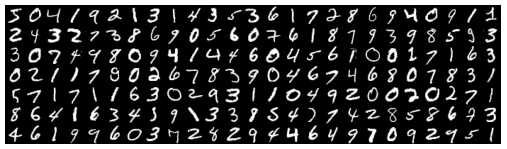
\includegraphics[width=\linewidth]{Pics/04_Data/MNIST.png}
    \caption{The first 175 samples of the MNIST data set of handwritten digits}
    \label{fig:MNISTdata175}
\end{figure}

\subsection{THETIS - Tennis shot videos}
The THETIS (Three dimEnsional TennIs Shots) data set consists of videos of 1980 tennis shots performed by both beginners and more experienced individuals \cite{Gourgari2013}. Each of the 12 types of shots types have been performed multiple times by each of the 55 individuals (31 beginners and 24 experts). Each shot consists of an RGB video, a depth video, a silhouette video, and both 2D and 3D skeleton videos. Since the skeleton extraction is not always successful, only 1217 of the shots have this feature. This means that the total number of videos in the data set is 8,374 resulting in a total playtime of 7 hours and 15 minutes. An overview of the 12 types of shots is given in \autoref{tab:typeOverviewTHETIS}, while an example of each of the five features is given in \autoref{fig:exampleVideosTennis}. 

\begin{table}
\centering
\caption{Overview of the 12 different types of tennis shots present in the THETIS data set.}
\label{tab:typeOverviewTHETIS}
\begin{tabular}{l|l|l|l}
\textbf{Forehand}    & \textbf{Backhand}     & \textbf{Service} & \textbf{Other} \\ \hline
Flat        & With 2 hands & Flat    & Smash \\
Slice       & Slice        & Slice   &       \\
Volley      & Volley       & Kick    &       \\
Open stands & Backhand     &         &      
\end{tabular}
\end{table}

\begin{figure}
    \centering
    \begin{subfigure}{.49\linewidth}
        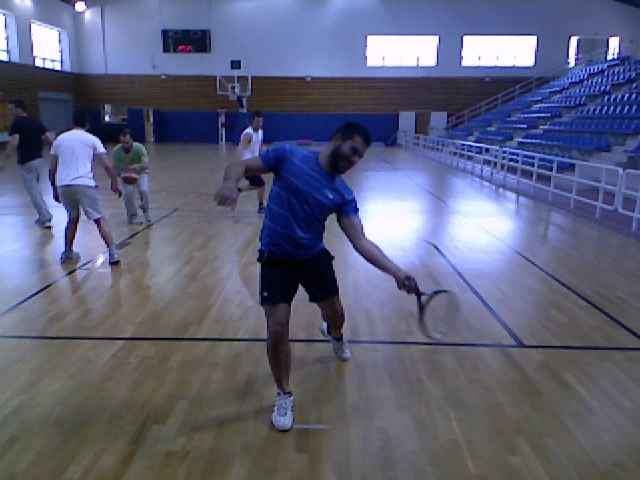
\includegraphics[width=\linewidth]{Pics/04_Data/frame53.jpg}
        \caption{Normal RGB video}
    \end{subfigure}
    \begin{subfigure}{.49\linewidth}
        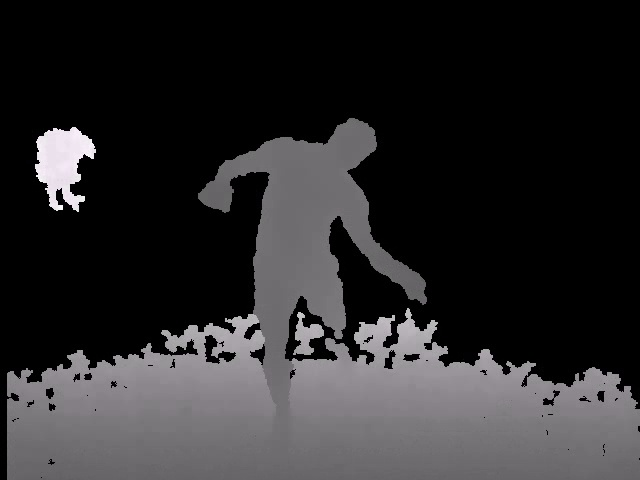
\includegraphics[width=\linewidth]{Pics/04_Data/frame53_depth.jpg}
        \caption{Depth video}
    \end{subfigure}
    \begin{subfigure}{.32\linewidth}
        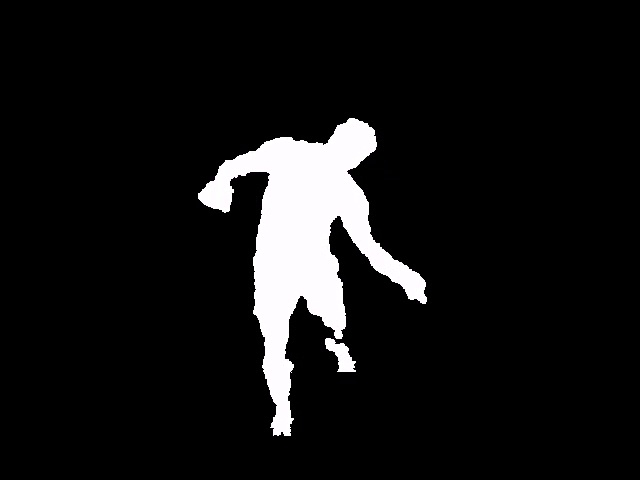
\includegraphics[width=\linewidth]{Pics/04_Data/frame53_mask.jpg}
        \caption{Silhouette}
    \end{subfigure}
    \begin{subfigure}{.32\linewidth}
        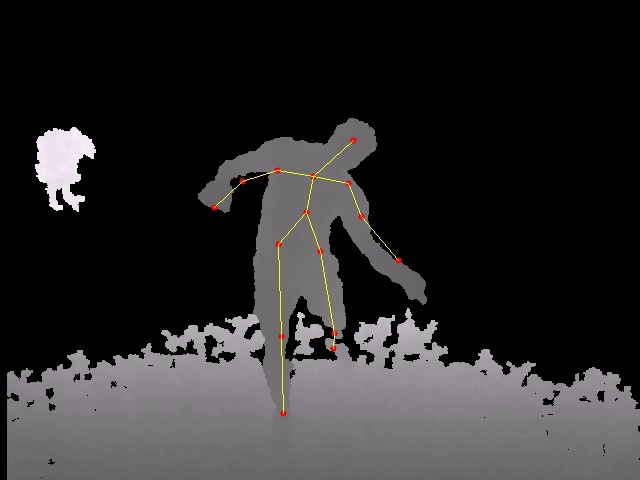
\includegraphics[width=\linewidth]{Pics/04_Data/frame53_skelet2D.jpg}
        \caption{2D Skeleton}
    \end{subfigure}
    \begin{subfigure}{.32\linewidth}
        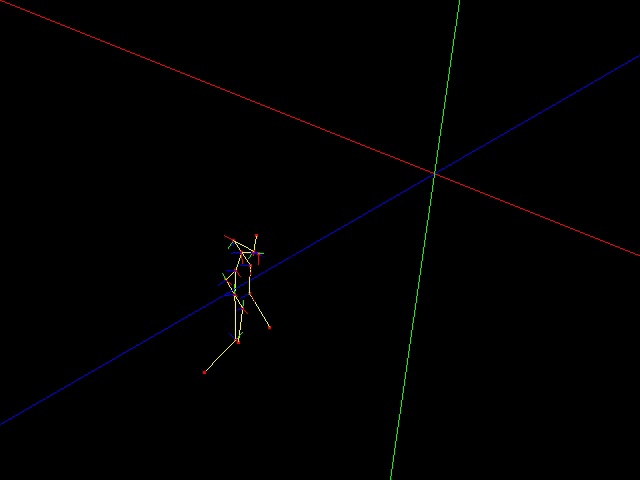
\includegraphics[width=\linewidth]{Pics/04_Data/frame53_skelet3D.jpg}
        \caption{3D skeleton}
    \end{subfigure}
    \caption{Example of the different videos that are given for each shot in the data set. Each of the pictures show the same frame in each of the videos of the same shot. Note that the 3D skeleton looks different since this is shown from a different angle. The 3D skeleton joint positions are also given numerically for each frame in the whole dataset.}
    \label{fig:exampleVideosTennis}
\end{figure}

Even though this data set is quite simple in relation to the real world, it is still complicated, especially with respect to the MNIST data set. The videos feature different individuals - both men and women, right handed and left handed, professionals and beginners. Even though the same type of shot is being performed by two individuals, they can look very different from each other. Also some of the videos are recorded in a sports arena with people doing different activities in the background as for instance yoga or basketball, while the others are recorded in a changing room with no noise at all.

\subsubsection{Pre-processing for THETIS}
As of now:
\begin{itemize}
    \item Put the depth video onto the RGB so it is now 4 input channels.
    \item Standardized length by manually assigning the middle of the shot and taking fixed number of frames on either side
    \item Decreased the resolution by a factor of 4 in each spatial dimension (factor of 16 overall)
\end{itemize}

\begin{figure}
    \centering
    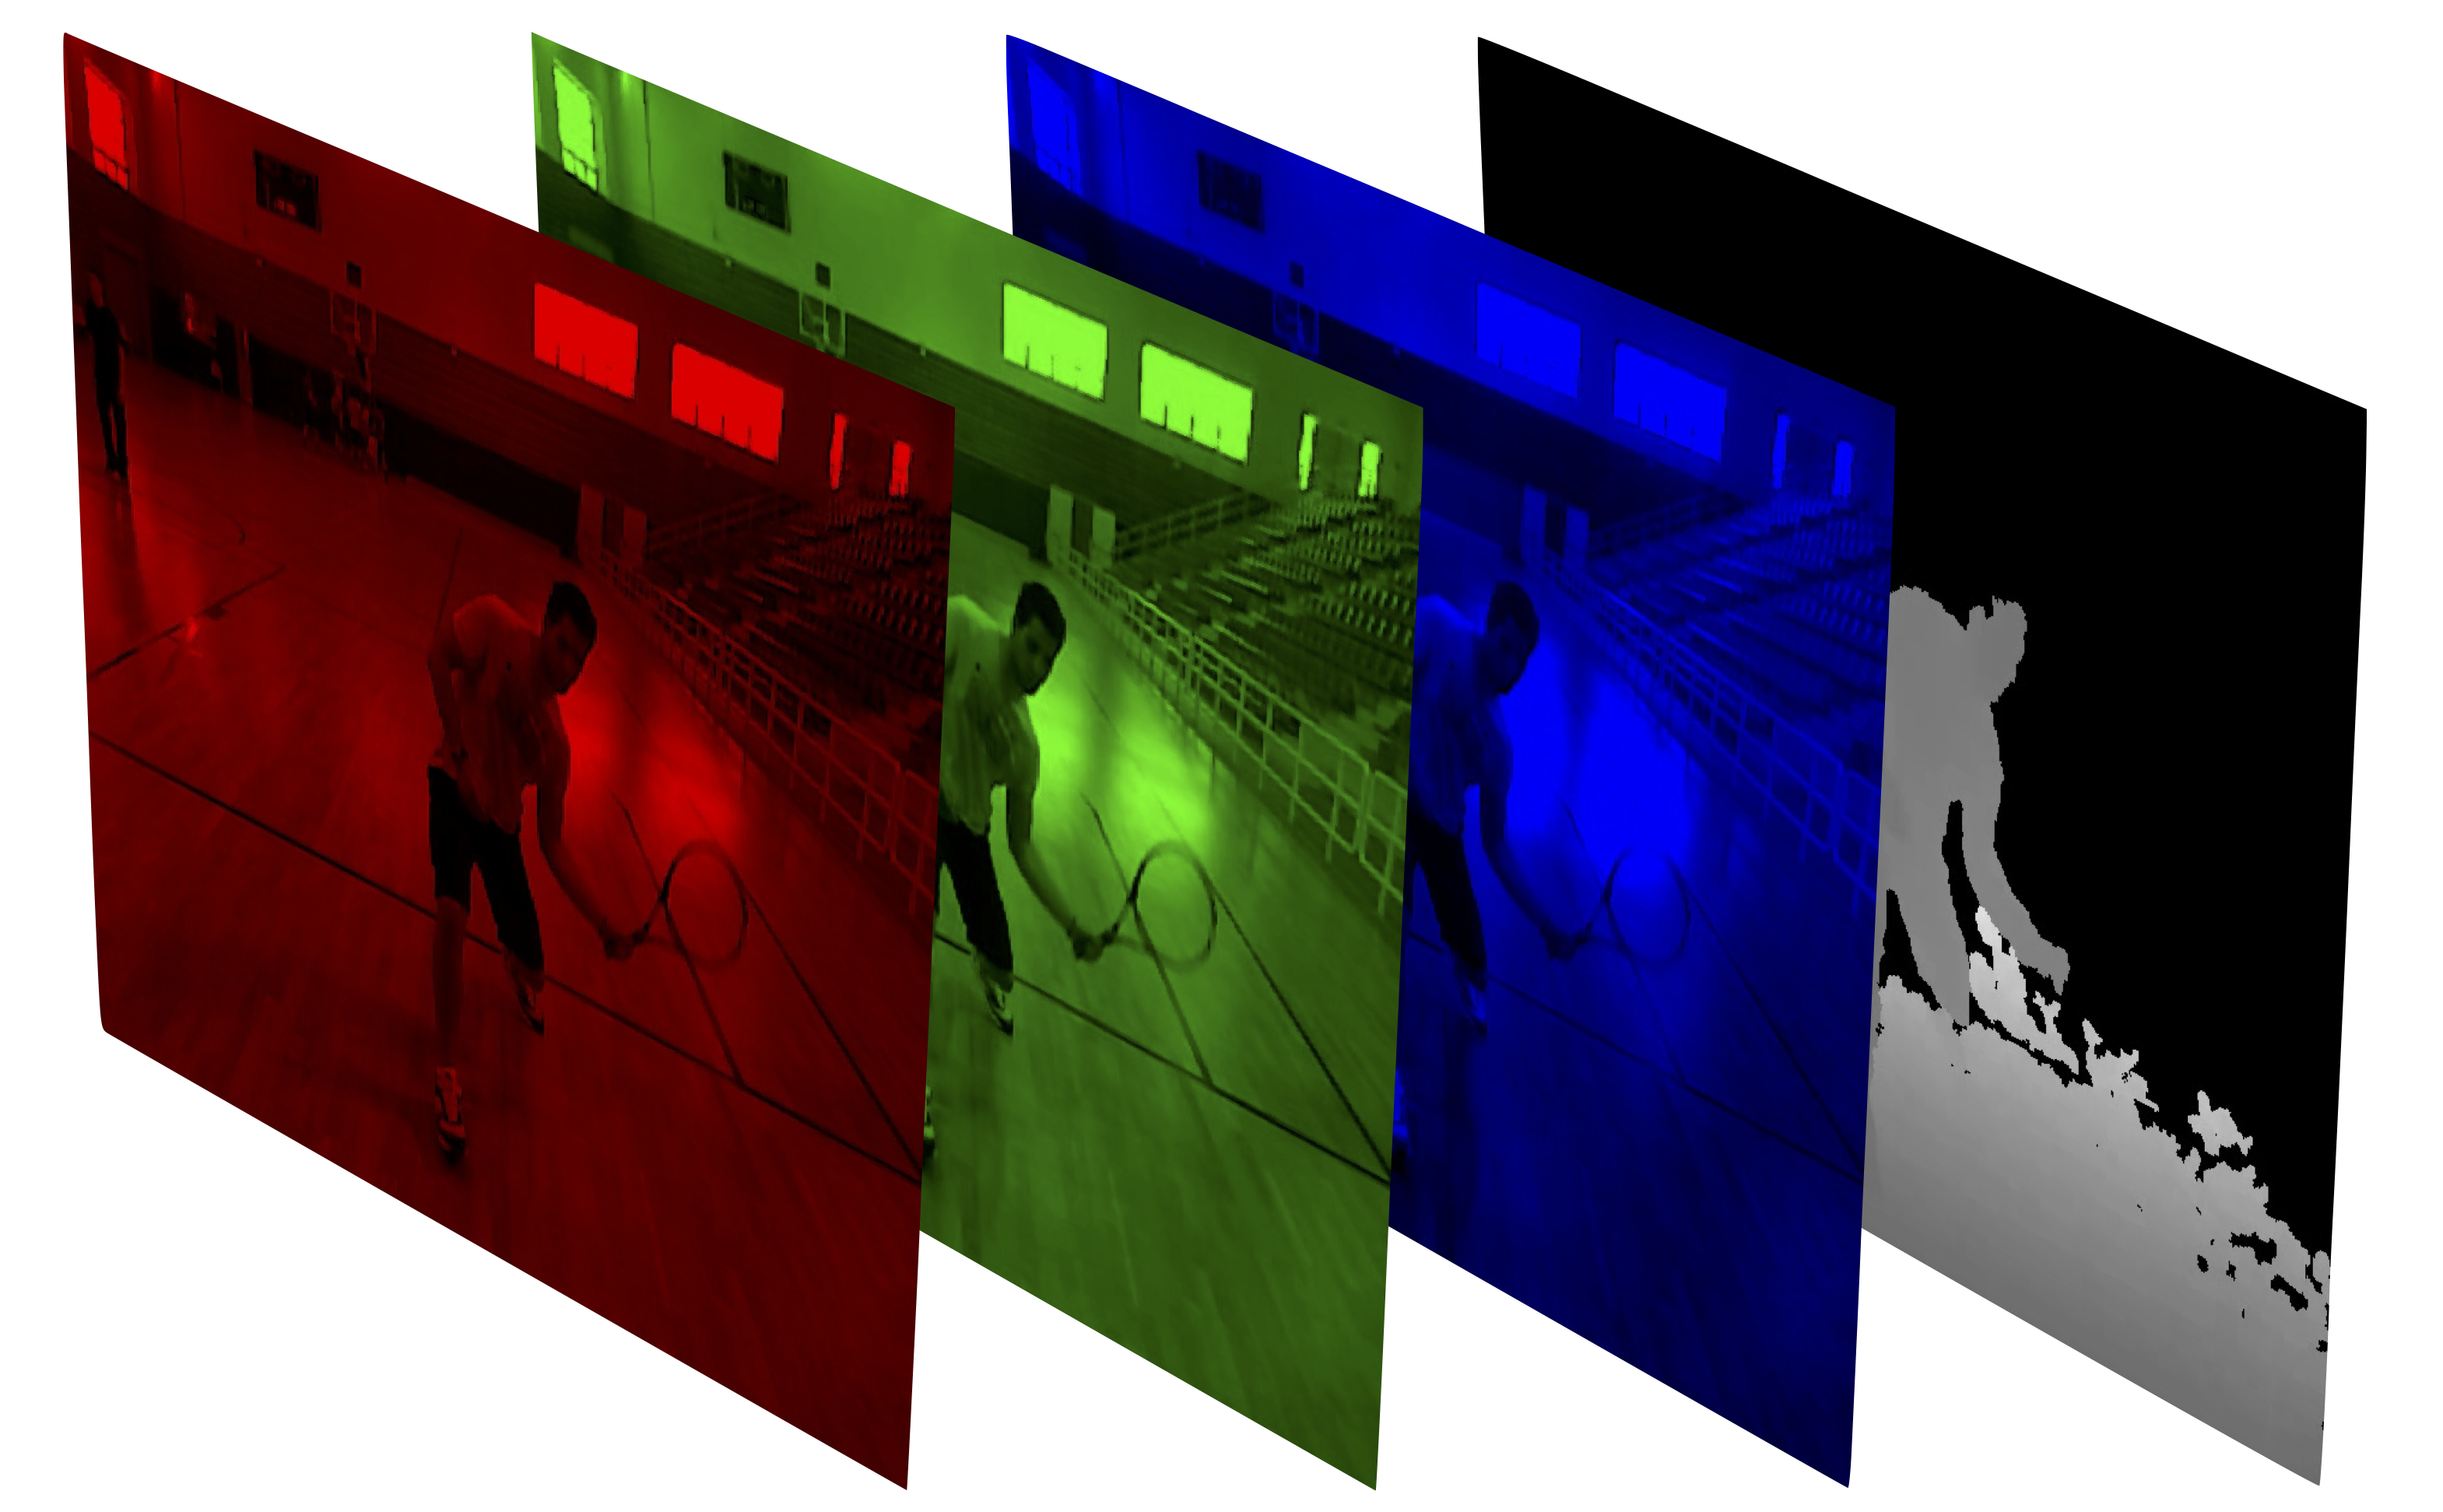
\includegraphics[width=.9\linewidth]{Pics/04_Data/RGBD.png}
    \caption{Each frame of the videos consists of 4 input channels; one red, one green, one blue, and one depth channel.}
    \label{fig:video_data_frame}
\end{figure}